\documentclass{article}

\usepackage{../repsty}

\usepackage{tikz}
\usetikzlibrary{trees, positioning, fit}
\usetikzlibrary{arrows, calc}
\usetikzlibrary{backgrounds}

\usepackage{amsfonts}
\usepackage{amsmath}
\usepackage{paralist}
\usepackage{soul}
\usepackage{color}

\usepackage{wrapfig}

\newcommand{\bias}[1]{\mathfrak{B}_{#1}}
\newcommand{\rand}[1]{\delta_{#1}}

\begin{document}
\title{Systematic Errors}
\author{Alexander Aksentyev}
\maketitle

\section*{Introduction}

The Test of Time-Reversal Invariance experiment (TRIC) is a transmission experiment aimed at achieving an accuracy in the order of $10^{-6}$ in the estimate of a cross section asymmetry. For that purpose, a polarized charged particle beam is scattered on a polarized target, and the rate of decay of the beam current is measured, which is proportional to the total scattering cross section. The difference in the cross sections for two opposite polarized states is proportional to the sought-after asymmetry. If the asymmetry is zero, Time-Reversal Invariance holds.

Here we will describe some possible problems with the experimental design that have to be overcome if one is to measure the asymmetry with a required accuracy.

\section{The Design}
In the following we describe the general idea of the experimental design of TRIC.

A particle beam circulates in the accelerator ring. At every turn it is scattered by the internal target at the rate $\CS[T]\Thick$, but there is also background loss happening in the ring at the rate $\CS[X]\Thick[X]$. (Notation: $\CS$ is the scattering cross section, $\Thick = \int_L n(z)\td z$ is the thickness of the scatterer, $L$ is the accelerator circumference.) At every turn the beam excites the current transformer (CT), and the average value of beam current is being recorded. 

All of this boils down to the following formula for the measured signal:
\[
	I_t  = I_0 \cdot e^{-\nu\bkt{\CS[T]\Thick + \CS[X]\Thick[X]}\cdot t} \equiv I_0\cdot e^{\slp\cdot t},
\]
where $\nu$ is the circulation frequency.

In TRIC, we use the deuterium target, and therefore it's polarization can be of either of two types: vector and tensor. The vector polarization $P^t_y$ aligns with the guiding magnetic field, as does the beam polarization (purely vector) $P_y$, and the tensor polarization $P^t_{xz}$ with the specially generated holding field in the target area.  The target cross section has the form
\begin{equation}\label{eq:CrossSection}
	\CS[T]^\pm = \CS[0]\cdot\bkt{1 + \Ayy P^t_y P^\pm + \Ayxz P^t_{xz} P^\pm}.
\end{equation}

The data are log-transformed, and the linear model $\ln I_t = \ln I_0 + \slp^\pm\cdot t + \err_t$ is fitted to it; the difference $\slp^- - \slp^+ = \nu\Thick\CS[0]\cdot\DP*\cdot\bkt{\Ayy P^t_y + \Ayxz P^t_{xz}}$. Ideally, the vector polarization component is $P^t_y = 0$, and we estimate the asymmetry as 
\begin{equation}\label{eq:AyxzEstimator}
\begin{cases}
	\Ayxz* 		&= \bkt{\nu\Thick\CS[0]\DP P^t_{xz}}^{-1}\cdot\bkt{\slp*^- - \slp*^+}, \\
	\SE{\Ayxz*} &= \bkt{\nu\Thick\CS[0]\DP P^t_{xz}}^{-1}\cdot\sqrt2\cdot\SE{\slp*}.
\end{cases}
\end{equation}

\newcommand{\Dt}{\Delta t}
Systematic deviations in the experimental conditions for the two spin states would modify the estimator in eq.~\eqref{eq:AyxzEstimator} in the following way:~\cite{DSPIN}
\begin{equation}\label{eq:AyxzAllBias}
	\Ayxz* = \Ayxz\bkt{1+\bias{\Dt}}\bkt*{1 + \bias{P_y} + \bias{P^t_{xz}}} + \Ayxz\bias{P^t_y},
\end{equation}
in which $\bias{\alpha}$ is the systematic difference in parameter $\alpha$ between the $+$ and $-$ experimental configurations, $\Dt$ is the beam current averaging time. Since the slope $\slp = \nu\Thick\CS[0]P_y\cdot\bkt{\Ayy P^t_y + \Ayxz P^t_{xz}}$, all the biases follow the simple expression:
\begin{equation}
	\bias{\alpha} = \frac{1}{\Ayxz}\frac{\partial\slp*}{\partial\alpha} \cdot \bkt{\alpha^- - \alpha^+}.
\end{equation}

\subsection{The AC/DC beam}
%The use of a bunched beam is preferable to that of the coasting beam because in the latter case the measurements have to be taken with an active current transformer. At the experimental energy, the beam makes $10^6$ revolutions per second, which implies three orders of magnitude more statistics with which to compute the average current, i.e. the measurement error is reduced by a factor of $30$.

A concern was raised, however, as to how the change from a DC beam to an AC one would affect the experimental methodology; if it would still be viable.

The estimation of the asymmetry requires fitting a model to a time series, and using a parameter of that model dependent on the asymmetry as the statistic. In our methodology, the model is log-linear. 

There are three elements to the measurement of the statistic: \begin{inparaenum}[1)]
	\item the beam interacting with the target,
	\item the measuring of the current by the CT, and
	\item the fitting of the data.
\end{inparaenum} 
So long as the beam's temporal structure does not affect the dynamics of the beam-target interaction, the latter two steps do not experience any structural change with the transition from a DC to an AC beam; the CT produces a discrete series of measurements in either case. The functional form of the CT signal is determined by the beam-target interaction dynamics, but as we assume it doesn't change, we have no ground on which to consider the statistical methodology viable for the DC beam doesn't remain such for the AC.
 
\section{Systematic errors}

We have estimated~\cite{Diploma} some of the bias terms in~\eqref{eq:AyxzAllBias}, and found them to be below $10^{-3}$. Besides, except the $\Ayxz\bias{P^t_y}$, all other biases are multiplied by the true value of the asymmetry, making them well below the required accuracy. The evaluation of $\Ayxz\bias{P^t_y}$ requires detailed knowledge of the distributions of the target gas density, and the holding magnetic field strength and direction, but the expressions for it will be provided in what follows.

%We will distinguish between two sources of systematic error when estimating a quantity: statistical methodology, and physical interpretation.
%
%The methodology source is the more easily accessible one; the errors of this kind are due to the contradiction between the assumptions made versus the properties of the data, and the latter can be easily checked. In essence, these errors arise from a lack of vigilance on the analysts' part.
%
%By an interpretation error, on the other hand, we mean a fundamental experimental design flaw, one that prohibits distinguishing between multiple channels the outcome could've come about.~\footnote{More on the subject of the schematic description of experiments in~\cite{Saunders}.}
%
%An example of a methodological systematic error would be using an ordinary least squares approach to fitting a time series with the autocorrelated disturbance term (generalized least squares are more appropriate here); or disregarding the fact that measurement error deterministically depends on time. 

%For an example of an interpretation error, consider the following: 

\subsection{The ideal conditions}
The ideal TRIC experiment requires that at least one of the two conditions hold: either
\begin{inparaenum}[1)]
	\item the injected ABS beam consists only of particles with the appropriate spin states, or
	\item the target chamber magnetic field does not have a vertical component.
\end{inparaenum}

Neither of the conditions are practically realizable, meaning that the vertical component of the target vector polarization is not zero. This means a beam particle can be scattered via either of \emph{two} channels which we have no way of distinguishing in our transmission experiment design. That means the estimator in~\eqref{eq:AyxzEstimator} must be corrected by subtracting a scaled estimate of $\Ayy$: 
\begin{equation}\label{eq:AyxzBiasCorrect}
\Ayxz* = C\Delta\slp* - \sfrac{P^t_y}{P^t_{xz}}\cdot\Ayy*.
\end{equation}
It also means the value of $\Ayy$ has to be estimated first, making TRIC a two-stage experiment.

%For an analysis of the statistical properties of the TRIC data obtained at COSY in 2016, please refer to~\cite{DAnaRep}. Below, we will concern ourselves with the interpretation problem outlined above.

\subsection{The holding field}

The target polarization is held oriented in the $xz$ direction of the horizontal plane by the holding magnetic field. The field's structure influences two aspects of the experiment's success: in the first place, the presence of a vertical component increases the magnitude of the bias term in eq.~\eqref{eq:AyxzBiasCorrect}; in the second, the deviation of the field's direction from 45 degrees in the horizontal plane decreases the magnitude of the useful signal.

\subsubsection{The increase of the faking signal}
The examination of the possible sources of systematic error~\cite{Proposal} shows that the vector-polarized total cross section scattering asymmetry $\Ayy$ is the primary source of systematic error in the reaction zone. The interfering scattering channel appears for two reasons: the inevitable presence of vector-polarized quantum states in the target's population, and the presence of the vertical component in the target chamber magnetic field. 

\begin{figure}[h]
	\centering
	\begin{subfigure}{.7\textwidth}
		\begin{tikzpicture}[scale=1]
		\node					(center)				{};
		
		\node					(x-axis)[above right=.5 and 2 of center] {$x$};
		\draw[->] (center) to (x-axis);
		\node					(y-axis)[above= 3 of center]	{$y$};
		\draw[->] (center) to (y-axis);
		\node					(z-axis)[below right=4 and13 of center] 	{$z$};
		\draw[->] (center) to (z-axis);
		
		\node		  (left vector) [above right=.5 and 3.25 of center]  {$B(-z)$};
		\draw[blue,dashed,->] (left vector) to +(1.5,-1.25);
		\node		  (right vector) at (10.,-.45) {$B(+z)$};
		\draw[blue,dashed,->] (right vector) to +(1.75,+1);
		\node (mid vector) at (7,-.75) {$B(0)$};
		\draw[blue,dashed,->] (mid vector) to +(2,-.1);
		
		\draw[blue,thick,>->] (5.5,2) .. controls (2,-1) and (14,-1) .. (10.5,1.75);
		%	\draw[red,dashed]		(4,.5) to (11,.5); % parallel line
		\draw[blue,thick,>->] (6,-2.85) .. controls (2,0) and (14,-1.) .. (10.5,-3.25);
				
		\coordinate[label=below right:cell] (A) at (5,-1); 
		\coordinate[label=below right:] (B) at (6.77,-.5); 
		
		\draw[dashed] (A) -- +(5,-1.5) -- +(5,.75) -- +(0,2) -- (A);
		\draw[dashed] (B) -- +(5,-1.5) -- +(5,.75) -- +(0,2) -- (B);
		\draw[dashed] (A) -- (B); \draw[dashed] (6.77,1.5) -- (5,1);
		\draw[dashed] (10,-2.5) -- (11.77,-2); \draw[dashed] (10,-.25) -- (11.77,.25);
		
		\end{tikzpicture}
		\caption{\label{fig:HoldingFld}}
	\end{subfigure}%
	\begin{subfigure}{.3\textwidth}
		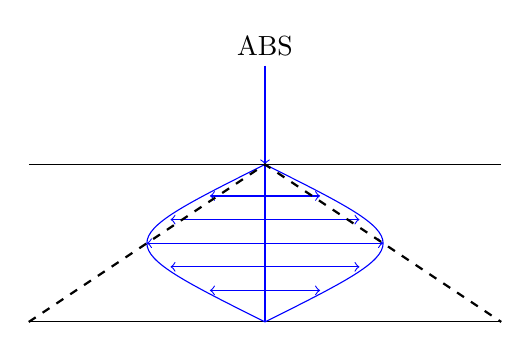
\begin{tikzpicture}[scale=1]
		\tikzstyle{vel} = [blue,->]
		\node (ctr) at (0,0) {}; \node (abs) at (0, 2.5) {ABS};
		\draw (-3, 1) -- (3,1);\draw(-3,-1) -- (3,-1);
		\draw[vel] (abs) -- (0,1);
		\draw[blue] (0,1) -- (0,-1); 
		\draw[blue] (0,1) .. controls (-2,0) .. (0,-1); 	\draw[blue] (0,1) .. controls (2,0) .. (0,-1); 
		
		\draw[vel] (0,0) -- (-1.5,0); \draw[vel] (0,0) -- (1.5,0);
		\draw[vel] (0,.3) -- (-1.2,.3); \draw[vel] (0,.3) -- (1.2,.3);
		\draw[vel] (0,.6) -- (-.7,.6); \draw[vel] (0,.6) -- (.7,.6);
		\draw[vel] (0,-.3) -- (-1.2,-.3); \draw[vel] (0,-.3) -- (1.2,-.3);
		\draw[vel] (0,-.6) -- (-.7,-.6); \draw[vel] (0,-.6) -- (.7,-.6);
		\draw[dashed,thick] (-3,-1) -- (0,1) -- (3,-1);
		\end{tikzpicture}
		\caption{\label{fig:VelDiag}}
	\end{subfigure}
	\caption{(a) Magnetic field lines of the holding field in the target chamber; (b) The gas number density distribution in the cell (dashed black line), and the velocity diagram (blue arrows).}
\end{figure}

In Figure~\ref{fig:HoldingFld} we drew a schematic representation of the structure of the holding field. According to it, the magnetic induction vector in the first half of the cell is related to that of the second half as in
\begin{align}
	\vec B(-z) &= (-B_x, -B_y, B_z)~\text{and}~\vec B(+z) = (B_x, B_y, B_z), \notag
\shortintertext{or}
	\vec B(-z) &= R(\hat{z}, \pi) \vec B(+z).
\end{align}
Since the spin vector aligns itself with the magnetic field, $P_y(-z) = -P_y(+z)$ too, so the minimization of the faking signal reduces to symmetrizing the holding field radially and along the $z$-direction. 

%One important aspect to consider is the fact that the field's vertical component tends to increase toward the cell edges; these are the areas where 

\subsubsection{The diminution of the true signal}
There's another aspect in which the magnetic field's structure influences eq.~\eqref{eq:AyxzBiasCorrect}. In order to have the maximum tensor polarization in the $xz$-direction, we need the horizontal component of the field be turned at 45 degrees to the side of the beam's orbit. It can be shown~\cite{Diploma} that the rate at which the beam scattering occurs is influenced by the field's inhomogeneity as in
\newcommand{\Lcell}{\ell}
\begin{equation}\label{eq:InhomogEffici}
		\slp = \slp'\cdot \frac{\int_{\Lcell}\rho(s)\cos2\Delta\Theta~\td s}{\int_{\Lcell}\rho(s)\td s},
\end{equation}
where $\Lcell$ is the cell length, $\rho(s)$ is the spatial distribution of the target density, and $\Delta\Theta$ is the angle deviation of the field's direction from 45 degrees. 

Simulation with parameters defined in Table~\ref{tbl:SpinFlip} indicate that the reaction efficiency can fall by as much as 70\%: $\slp = 0.31\cdot \slp'$.

\subsection{Spin flipping}
There are two possible ways to perform the time-reversed $\vec{p}\vec{d}$ scattering: we can flip the beam's polarization, or we can flip the target's. If we do the latter, this is accomplished by inverting the direction of the magnetic field. However, in this case we would have to ensure that the inverted field's deviation from the desired direction is not systematically different from the original. If it is (and it's likely to be), the scattering efficiencies of the two cases would be different, and a bias would be introduced.

Let us denote the angle deviation at a point $z$ $\Delta\theta(z) = \bias{\theta} + \rand{\theta}$. Then the bias one can expect in the estimate $\Ayxz*$ is~\cite{Diploma}
\begin{equation}\label{eq:FlipEfficiBias}
	\bias{\Ayxz*} = \frac{1}{2}\bkt*{F\bkt{\Xpct{A(\chi^c)}\cos2\bias{\theta}^+} + F\bkt{\Xpct{A(\chi^c)}\cos2\bias{\theta}^-}} - 1,
\end{equation}
where $F(f) = \sfrac{1}{\Thick[T]}\cdot\int_{\Lcell}\rho(z) f(z)~ \td z$, $\chi^c$ a measure of the magnetic field strength, $A(\chi^c)$ is the proportionality coefficient between the magnetic field strength and the target polarization.

Estimates with an assumed parabolic distribution $\Delta\theta(z)$ show the bias in~\eqref{eq:FlipEfficiBias} to be in the order of $5\cdot 10^{-4}\cdot\Ayxz$ for the parameters shown in Table~\ref{tbl:SpinFlip}.~\cite{Diploma} 

\begin{center}
	\begin{threeparttable}
		\centering
		\caption{The model assumed for modeling the effects of the holding field inhomogeneity. \label{tbl:SpinFlip}}
		\begin{tabular}{crr}
			\hline\hline
			Parameter     &              Cell center &                Cell edge \\ \hline
			$\Delta\theta(z)$ &               $45^\circ$ &                $5^\circ$ \\
			$\rho(z)$     & $3\cdot10^{12}~ at/cm^3$ & $1\cdot 10^{12}~at/cm^3$ \\ \hline
		\end{tabular}
		\begin{tablenotes}
			\item $\rho(z)$ is the target density (plotted in Figure~\ref{fig:VelDiag}), and $\Delta\theta$ is the angular deviation of the holding field from 45 $^\circ$ in the $xz$-plane.
		\end{tablenotes}
	\end{threeparttable}
\end{center}



\section*{Conclusion}
In this report we've summarized the goal and design of TRIC. The general form of the total cross section asymmetry estimator in the presence of systematic errors has been given (eq.~\eqref{eq:AyxzAllBias}), and the upper bound on the multiplicative biases was estimated ($10^{-3}\cdot\Ayxz$). The additive bias, the major source of systematic error in this experiment, was considered separately. 

It is difficult to estimate this bias without knowledge of the distributions of the gas density and the holding field in the cell (their symmetry ultimately determines the magnitude of the vertical component of the target vector polarization), but from eq.~\eqref{eq:AyxzBiasCorrect} we know that whatever those are, one requires both the prior estimate $\Ayy*$ and the ratio $r = \sfrac{P^t_y}{P^t_{xz}}$ to be known sufficiently well to satisfy
\begin{equation}
	\sqrt{r^2 \cdot\SE{\Ayy*}^2 + \Ayy^2\SE{r}^2 + \SE{\Ayy*}^2\cdot\SE{r}^2} \leq 1\cdot10^{-6}.
\end{equation}

The holding field influences the success of the experiment in another way: the efficiency of the tensor-polarized scattering of the beam on the target is encapsulated in eq.~\eqref{eq:InhomogEffici}. As the holding field deviates from its nominal direction of 45$^\circ$ in the horizontal plane, the $xz$-component of the target tensor polarization diminishes, and the measurements become more susceptible to the faking signal.

Time-reversal can be performed by inverting the direction of the target chamber magnetic field. In that case, if the field inhomogeneity differs for the opposite field configurations, an efficiency bias is introduced, described by eq.~\eqref{eq:FlipEfficiBias}. Estimates obtained by modeling with parameters summarized in Table~\ref{tbl:SpinFlip} indicate that this bias should be four orders of magnitude below the value of the $\Ayxz$ itself.

\begin{thebibliography}{9}
	\bibitem{DSPIN}
	Yury Valdau, Alexander Aksentyev, Dieter Eversheim, and Bernd Lorentz. ``The Physics Program of PAX at COSY.'' IOP Publishing, Conference Series, 678 (2016).
	
	
%	\bibitem{Saunders}
%	Simon Saunders. ``Derivation of the Born Rule from Operational Assumptions.'' arXiv:quant-Ph/0211138, November 21, 2002. \url{http://arxiv.org/abs/quant-ph/0211138.}
		
	\bibitem{Proposal}
	P.D. Eversheim, B. Lorentz, and Yu. Valdau, Forschungszentrum J\"ulich, COSY, proposal \#215, 2012.
	
	\bibitem{Diploma}
	Alexander Aksentyev. Diploma thesis (2015).
	
	\bibitem{DAnaRep}
	Alexander Aksentyev. ``Analysis of the 2016 data.''
\end{thebibliography}



\end{document}